\documentclass[aspectratio=169]{beamer}

% Use metropolitan theme
\usetheme{metropolis}

% Packages
\usepackage{booktabs}
\usepackage{colortbl, comment}

% Title page information
\title{The Virtue of Complexity in Simple Economic Models}

\author{Kerry Back \and Alexander Ober \and Seth Pruitt}


\date{}

% Footer setup
\setbeamertemplate{frame numbering}[fraction]
\setbeamertemplate{footline}{
  \begin{beamercolorbox}[wd=\textwidth,ht=3ex,dp=1.5ex,leftskip=0.3cm,rightskip=0.3cm]{structure}
    UTEP, Feb 2026
    \hfill
    \insertframenumber{} / \inserttotalframenumber
  \end{beamercolorbox}
}

\begin{document}

% Title slide
\begin{frame}
  \titlepage
\end{frame}

% Overview slide
\begin{frame}{Overview}

  \begin{itemize}
    \item Recent work by Bryan Kelly, Semyon Malamud and co-authors argue that there is a ``virtue of complexity'' in empirical asset pricing, meaning we should use models with many, many factors.
    \item This (perhaps) runs counter to the standard practice of seeking parsimonious models. 
    \item The theoretical part of their work has generated some controversy.
    \item We focus on the empirical part and ask: does complexity work because the world is complex or does it work even in simple environments?
  \end{itemize}
\end{frame}

\begin{frame}{Simple Economic Models}
\begin{itemize}
\item We simulate data from three theoretical models: Berk-Green-Naik (1999), Kogan-Papanikolaou (2014), Gomes-Schmid (2021)
\item All are equilibrium models that generate a panel of firms with varying characteristics and expected returns.
\begin{itemize}
\item Expected returns depend on covariances with a stochastic discount factor
\item Covariances are correlated in the cross-section with characteristics
\end{itemize}
\item We evaluate the complexity method by
\begin{itemize}
\item Determining whether performance improves as complexity increases
\item Comparing complex models to Fama-French, Fama-MacBeth, and the CAPM.
\end{itemize}
\end{itemize}
\end{frame}


\begin{frame}{Didisheim-Ke-Kelly-Malamud Characteristic Factors}

\begin{itemize}
  \item Factors = returns of portfolios whose weights are rank-standardized characteristic values in $[-0.5, 0.5]$
  \item Example: book-to-market factor would be return of portfolio that is long value stocks (above median bm) and short growth stocks (below median bm).
  \item "More value" $\Rightarrow$ higher weight.  "More growth" $\Rightarrow$ more negative weight.
\end{itemize}
\end{frame}

\begin{frame}{Composite Characteristics and Factors}
\begin{itemize}
  \item Start with $M$ characteristics $c_{ik}$.  Generate $M$ random numbers $h_k$.  Compute two new composite characteristics
$$\cos\left(\sum_{k=1}^M h_kc_{ik}\right) \quad \text{and} \quad \sin\left(\sum_{k=1}^M h_kc_{ik}\right)$$
  \item Repeat many times to get thousands of new composite characteristics.
  \item Define a factor as described before for each of the new composite characteristics
\end{itemize}
\end{frame}

\begin{frame}{DKKM Empirical Results}
\begin{itemize}
  \item 130 stock characteristics
  \item Out-of-sample Sharpe ratios reach 4.0 with high-complexity models (10,000+ factors)
   \item Fama-French-Carhart 6-factor Sharpe ratio $\approx$ 1.1
 \end{itemize}
\end{frame}

\begin{frame}[c]
  \centering
  \Huge Data-Generating Models
\end{frame}

\begin{frame}{Theoretical Models: Overview}
\begin{itemize}
\item In all models, risk premia depend on covariances with a stochastic discount factor.
\item In all models, the covariances are correlated in the cross-section with firm characteristics.
\item Hence, characteristics `explain' risk premia.
\item In all models, we can compute size, book-to-market, profitability, asset growth, and momentum (the FFC6 characteristics).
\item We can also compute the true \alert{traded} stochastic discount factor and the true tangency portfolio.
\end{itemize}
\end{frame}

\begin{frame}{Berk, Green, and Naik (1999)}
\begin{itemize}
  \item Firms invest optimally given an exogenous pricing kernel
  \item Fixed number of firms, each receives take-it-or-leave-it investment opportunities each period
  \item Projects generate operating cash flows until they randomly die
  \item Investment depends on project NPV (which varies with beta and interest rates)
  \item Model generates: book value, market value, net income, stock returns
  \item Characteristics: size, book-to-market, ROE, asset growth, momentum
\end{itemize}
\end{frame}

\begin{frame}{Kogan and Papanikolaou (2014)}
\begin{itemize}
  \item Firms invest optimally given an exogenous pricing kernel
  \item Two aggregate state variables:
  \begin{itemize}
    \item Disembodied productivity affecting all capital
    \item Productivity of newly installed capital
  \end{itemize}
  \item Firms acquire projects stochastically at firm-specific rates
  \item Optimal capital investment choice for each project
  \item Firm-specific and project-specific productivity processes
  \item Projects produce cash flows until they randomly expire
\end{itemize}
\end{frame}

\begin{frame}{Gomes and Schmid (2021)}
\begin{itemize}
  \item General equilibrium model with heterogeneous firms
  \item Representative household with Epstein-Zin preferences (endogenous SDF)
  \item Firms make optimal investment and financing decisions
  \item Single aggregate productivity process (AR(1)) + firm-specific shocks
  \item Stochastic investment opportunities with random costs
  \item Lumpy investment (discrete project adoption)
  \item Debt: consol bonds paying coupons until random expiration
  \item Tax benefits of debt; costly equity issuance (pecking order)
  \item Strategic default when equity value $\leq 0$
\end{itemize}
\end{frame}


\begin{frame}[c]
  \centering
  \Huge Our Simulations
\end{frame}

\begin{frame}{Advantage of Simulations}
  \begin{itemize}
  \item Can compute true conditional expected returns, risks, and Sharpe ratios
  \item Can compute true traded SDF
  \item Can compute 
  $$(\text{estimated SDF value}-\text{true SDF value})^2$$
   each period - the foundation of the Hansen-Jagannathan distance
  \end{itemize}

\end{frame}

\begin{frame}{Simulation Design}
\begin{itemize}
  \item 1,000 firms and 920 months in each panel (discard first 200 as burn-in, leaving 60 years)
  \item 12 independent panels for each data-generating model
  \item In each panel for each model in each month, compute true conditional SDF and true conditional max Sharpe ratio
  \item Use calibrations from original papers, except we substitute exogenous lognormal SDF in Gomes-Schmid, calibrated to match market risk premium
\end{itemize}
\end{frame}


\begin{frame}{Evaluations of Empirical Methods}

\begin{itemize}
\item Compare conditional Sharpe ratios of estimated MVE portfolios of factors

\vspace{0.4cm}
\begin{quote}
\leftskip=2em\rightskip=2em
\upshape Barillas-Shanken, 2017: in horse race between factor models, assuming test assets include competing factors, model with highest Sharpe ratio wins
\end{quote}
\item Estimate conditional SDFs implied by the models and compute Hansen-Jagannathan distance to true conditional SDF

\vspace{0.4cm}
\begin{quote}
\leftskip=2em\rightskip=2em
\upshape HJ distance is the maximum pricing error over all test assets with unit uncentered second moment
\end{quote}
\item Look at pricing errors for 25 size and book-to-market sorted portfolios
\end{itemize}
\end{frame}

\begin{frame}{Britten-Jones Regression}
  \begin{itemize}
\item Can find empirical mean-variance frontier by linear regression of constant 1 on asset excess returns
\item Write fitted regression as
\begin{align*}
1 &=  \sum_{i=1}^N \hat \beta_i (r_{i}-r_{f}) + \hat \varepsilon \\
&= \hat z + \hat \varepsilon
\end{align*}
\item Max Sharpe ratio is $\bar z/ \sigma_z$
\item Result originally due to Hansen and Richard for population: projection in population rather than regression in sample
\end{itemize}
\end{frame}

\begin{frame}{Britten-Jones Regression}
  \centering
  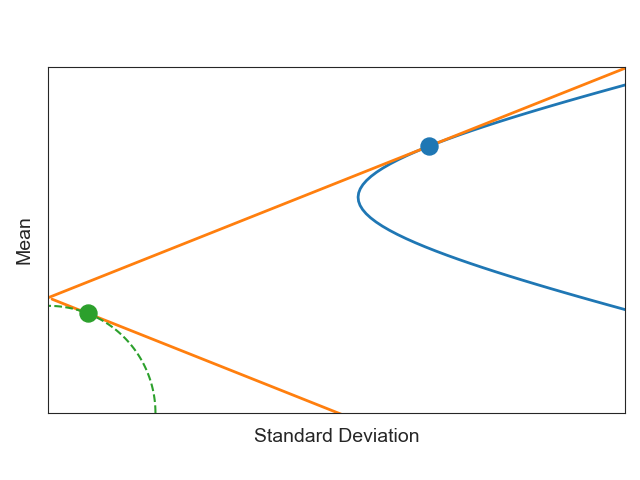
\includegraphics[height=0.6\textheight]{meanvar.png}

\vspace{-0.2cm}
\begin{itemize}
\item Green dot $= r_f - (1+r_f) \hat z = $ SDF scaled to be a gross return $-1$
\item Tangency portfolio return $= rf + \lambda z$ for some $\lambda >0$
\end{itemize}
\end{frame}

\begin{frame}{Our Implementation}
\begin{itemize}
\item Use known true distributions to calculate $\hat \varepsilon$.  Use as SDF (orthogonal to excess returns).
\item In empirical factor models, use Britten-Jones regression on rolling 360 month windows (following DKKM)
\item With many factors (maybe more than 360), use ridge penalization in Britten-Jones regression (following DKKM)
\end{itemize}
\end{frame}

\begin{frame}{Performance Measures for Each Factor Model}
\begin{itemize}
\item Mean theoretical conditional max Sharpe ratio in each panel
\item Realized HJ distance: Square root of mean value of $(\hat \varepsilon_{\text{factors}} - \hat \varepsilon_{\text{all-returns}})^2$ in each panel
\item GRS statistic and max Sharpe ratio of unspanned returns of 25 size and book-to-market sorted portfolios
\end{itemize}
\end{frame}

\begin{frame}{Ridge Regression}
\begin{itemize}
  \item Minimize: $\frac{1}{T}\sum_{t=1}^T (1 - \beta' F_t)^2 + \alpha \beta'\beta$
  \item Penalty parameter $\alpha$ controls shrinkage toward zero
  \item Essential when number of factors $M$ is large relative to sample size $T$
  \item We examine performance for various $\alpha$
\end{itemize}
\end{frame}

\begin{frame}{Empirical Factors}
\begin{itemize}
\item Form factors from size, book-to-market, operating profitability, asset growth, and momentum in all models
\item Fama-French-Carhart (FFC): usual $2\times 3$ sorts, use size/book-to-market sort to form SMB
\item Fama-MacBeth-Rosenberg (FMR): Fama-MacBeth regressions on characteristics
\item Didisheim-Ke-Kelly-Malamud (DKKM): random Fourier features built from the five characteristics plus market return (not penalized in ridge)
\item In Berk-Green-Naik, include risk-free rate among DKKM characteristics
\item In Gomes-Schmid, include leverage in all methods (for FFC, $2\times 3$ sort on size and leverage)
\end{itemize}
\end{frame}

\begin{frame}{Fama-MacBeth-Rosenberg}
\begin{itemize}
  \item Fama-MacBeth (1973), Rosenberg (1976), Fama (1976)
  \item Regression coefficients $(X'X)^{-1}X'R$ are linear combinations of returns $R$
  \item Set $W = X(X'X)^{-1}$ so regression coefficients are $W'y$
  \item Regression coefficients are payoffs of portfolios constituting the columns of $W$
\end{itemize}
\end{frame}

\begin{frame}{Diversification Property}
\begin{itemize}
  \item \# columns $W=$ \# characteristics $+1$.  $W$ satisfies $X'W=I$
  \item Each portfolio has a unit inner product with the corresponding column of $X$ and is orthogonal to other columns
  \item Except for the first (intercept) portfolio, each portfolio is a zero-investment portfolio with a unit value for one characteristic and a zero value for all others.
  \item Many solutions $W$ of $X'W=I$, but projection $W=X(X'X)^{-1}$ solves, for each column, $\min \; w'w$ subject to orthonormal constraint
  \item We rescale so long and short sides each sum to 1.
\end{itemize}
\end{frame}


\begin{frame}[c]
  \centering
  \Huge Results
\end{frame}

\begin{comment}
\begin{frame}{BGN Model: Sharpe Ratios}
  \centering
  \begin{columns}
    \begin{column}{0.45\textwidth}
      \centering
      \begin{tabular}{l c}
\toprule
Method & Sharpe Ratio \\
\midrule
True SDF & 0.65 \\
\midrule
CAPM & 0.20 \\
FFC & 0.36 \\
FMR & 0.37 \\
DKKM & 0.43 \\
\bottomrule
\end{tabular}
    \end{column}
    \begin{column}{0.55\textwidth}
      \centering
      \begin{tabular}{l c c c c}
\toprule
$\alpha$ & 6 & 36 & 360 & 3600 \\
\midrule
0 & 0.400 & 0.405 & 0.019 & 0.189 \\
0.001 & 0.399 & 0.422 & 0.404 & 0.402 \\
0.01 & 0.394 & 0.426 & 0.429 & 0.428 \\
0.05 & 0.379 & 0.410 & 0.414 & 0.414 \\
0.1 & 0.365 & 0.393 & 0.397 & 0.397 \\
1.0 & 0.283 & 0.291 & 0.292 & 0.292 \\
\bottomrule
\end{tabular}

      \vspace{0.2cm}
      \small DKKM by $\alpha$ and \# factors
    \end{column}
  \end{columns}
\end{frame}

\begin{frame}{BGN Model: HJ Distance}
  \centering
  \begin{columns}
    \begin{column}{0.45\textwidth}
      \centering
      \begin{tabular}{l c}
\toprule
Method & HJ Distance \\
\midrule
CAPM & 0.50 \\
FFC & 0.43 \\
FMR & 0.51 \\
DKKM & 0.39 \\
\bottomrule
\end{tabular}
    \end{column}
    \begin{column}{0.55\textwidth}
      \centering
      \begin{tabular}{l c c c c}
\toprule
$\alpha$ & 6 & 36 & 360 & 3600 \\
\midrule
0 & 0.407 & 0.439 & 21.959 & 1.563 \\
0.001 & 0.407 & 0.415 & 0.428 & 0.434 \\
0.01 & 0.409 & 0.396 & 0.388 & 0.388 \\
0.05 & 0.417 & 0.398 & 0.393 & 0.393 \\
0.1 & 0.427 & 0.408 & 0.405 & 0.406 \\
1.0 & 0.472 & 0.468 & 0.468 & 0.468 \\
\bottomrule
\end{tabular}

      \vspace{0.2cm}
      \small DKKM by $\alpha$ and \# factors
    \end{column}
  \end{columns}
\end{frame}

\begin{frame}{KP14 Model: Sharpe Ratios}
  \centering
  \begin{columns}
    \begin{column}{0.45\textwidth}
      \centering
      \begin{tabular}{l c}
\toprule
Method & Sharpe Ratio \\
\midrule
True SDF & 0.24 \\
\midrule
CAPM & 0.12 \\
FFC & 0.19 \\
FMR & 0.18 \\
DKKM & 0.21 \\
\bottomrule
\end{tabular}
    \end{column}
    \begin{column}{0.55\textwidth}
      \centering
      \begin{tabular}{l c c c c}
\toprule
$\alpha$ & 6 & 36 & 360 & 3600 \\
\midrule
0 & 0.195 & 0.136 & 0.003 & 0.014 \\
0.001 & 0.197 & 0.168 & 0.153 & 0.151 \\
0.01 & 0.202 & 0.195 & 0.193 & 0.192 \\
0.05 & 0.205 & 0.207 & 0.207 & 0.207 \\
0.1 & 0.204 & 0.207 & 0.207 & 0.207 \\
1.0 & 0.180 & 0.184 & 0.184 & 0.183 \\
\bottomrule
\end{tabular}

      \vspace{0.2cm}
      \small DKKM by $\alpha$ and \# factors
    \end{column}
  \end{columns}
\end{frame}

\begin{frame}{KP14 Model: HJ Distance}
  \centering
  \begin{columns}
    \begin{column}{0.45\textwidth}
      \centering
      \begin{tabular}{l c}
\toprule
Method & HJ Distance \\
\midrule
CAPM & 0.23 \\
FFC & 0.19 \\
FMR & 0.20 \\
DKKM & 0.17 \\
\bottomrule
\end{tabular}
    \end{column}
    \begin{column}{0.55\textwidth}
      \centering
      \begin{tabular}{l c c c c}
\toprule
$\alpha$ & 6 & 36 & 360 & 3600 \\
\midrule
0 & 0.180 & 0.290 & 20.202 & 1.032 \\
0.001 & 0.178 & 0.223 & 0.250 & 0.254 \\
0.01 & 0.172 & 0.180 & 0.183 & 0.183 \\
0.05 & 0.170 & 0.167 & 0.167 & 0.167 \\
0.1 & 0.171 & 0.167 & 0.167 & 0.167 \\
1.0 & 0.197 & 0.194 & 0.194 & 0.194 \\
\bottomrule
\end{tabular}

      \vspace{0.2cm}
      \small DKKM by $\alpha$ and \# factors
    \end{column}
  \end{columns}
\end{frame}

\begin{frame}{GS21 Model: Sharpe Ratios}
  \centering
  \begin{columns}
    \begin{column}{0.45\textwidth}
      \centering
      \begin{tabular}{l c}
\toprule
Method & Sharpe Ratio \\
\midrule
True SDF & 2.26 \\
\midrule
CAPM & 0.02 \\
FFC & 1.55 \\
FMR & 1.55 \\
DKKM & 1.77 \\
\bottomrule
\end{tabular}
    \end{column}
    \begin{column}{0.55\textwidth}
      \centering
      \begin{tabular}{l c c c c}
\toprule
$\alpha$ & 6 & 36 & 360 & 3600 \\
\midrule
0 & 1.634 & 1.828 & 0.194 & 0.223 \\
1e-5 & 1.634 & 1.827 & 1.674 & 1.591 \\
1e-4 & 1.634 & 1.814 & 1.760 & 1.738 \\
5e-4 & 1.634 & 1.789 & 1.777 & 1.772 \\
0.001 & 1.633 & 1.777 & 1.773 & 1.772 \\
0.01 & 1.618 & 1.751 & 1.759 & 1.760 \\
\bottomrule
\end{tabular}

      \vspace{0.2cm}
      \small DKKM by $\alpha$ and \# factors
    \end{column}
  \end{columns}
\end{frame}

\begin{frame}{GS21 Model: HJ Distance}
  \centering
  \begin{columns}
    \begin{column}{0.45\textwidth}
      \centering
      \begin{tabular}{l c}
\toprule
Method & HJ Distance \\
\midrule
CAPM & 0.91 \\
FFC & 0.44 \\
FMR & 0.47 \\
DKKM & 0.34 \\
\bottomrule
\end{tabular}
    \end{column}
    \begin{column}{0.55\textwidth}
      \centering
      \begin{tabular}{l c c c c}
\toprule
$\alpha$ & 6 & 36 & 360 & 3600 \\
\midrule
0 & 0.437 & 0.315 & 7.230 & 1.155 \\
1e-5 & 0.438 & 0.317 & 0.363 & 0.397 \\
1e-4 & 0.438 & 0.326 & 0.336 & 0.343 \\
5e-4 & 0.439 & 0.342 & 0.340 & 0.341 \\
0.001 & 0.440 & 0.350 & 0.347 & 0.347 \\
0.01 & 0.454 & 0.380 & 0.375 & 0.375 \\
\bottomrule
\end{tabular}

      \vspace{0.2cm}
      \small DKKM by $\alpha$ and \# factors
    \end{column}
  \end{columns}
\end{frame}
\end{comment}

\begin{frame}{Berk-Green-Naik Model}
  \centering
  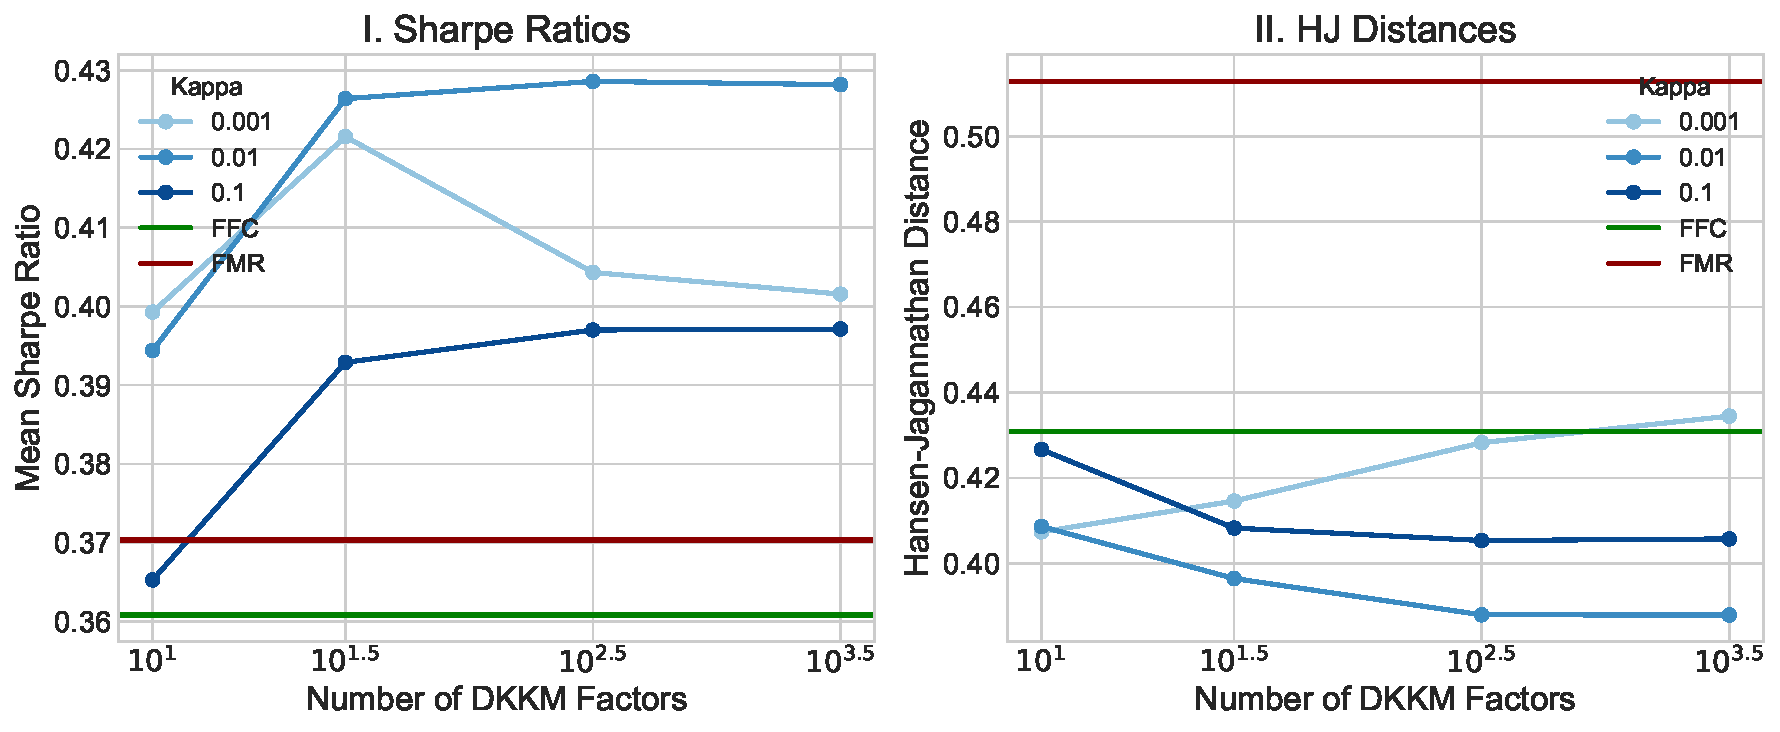
\includegraphics[width=\textwidth]{figures/dkkm_bgn.pdf}
\end{frame}

\begin{frame}{Kogan-Papanikolaou Model}
  \centering
  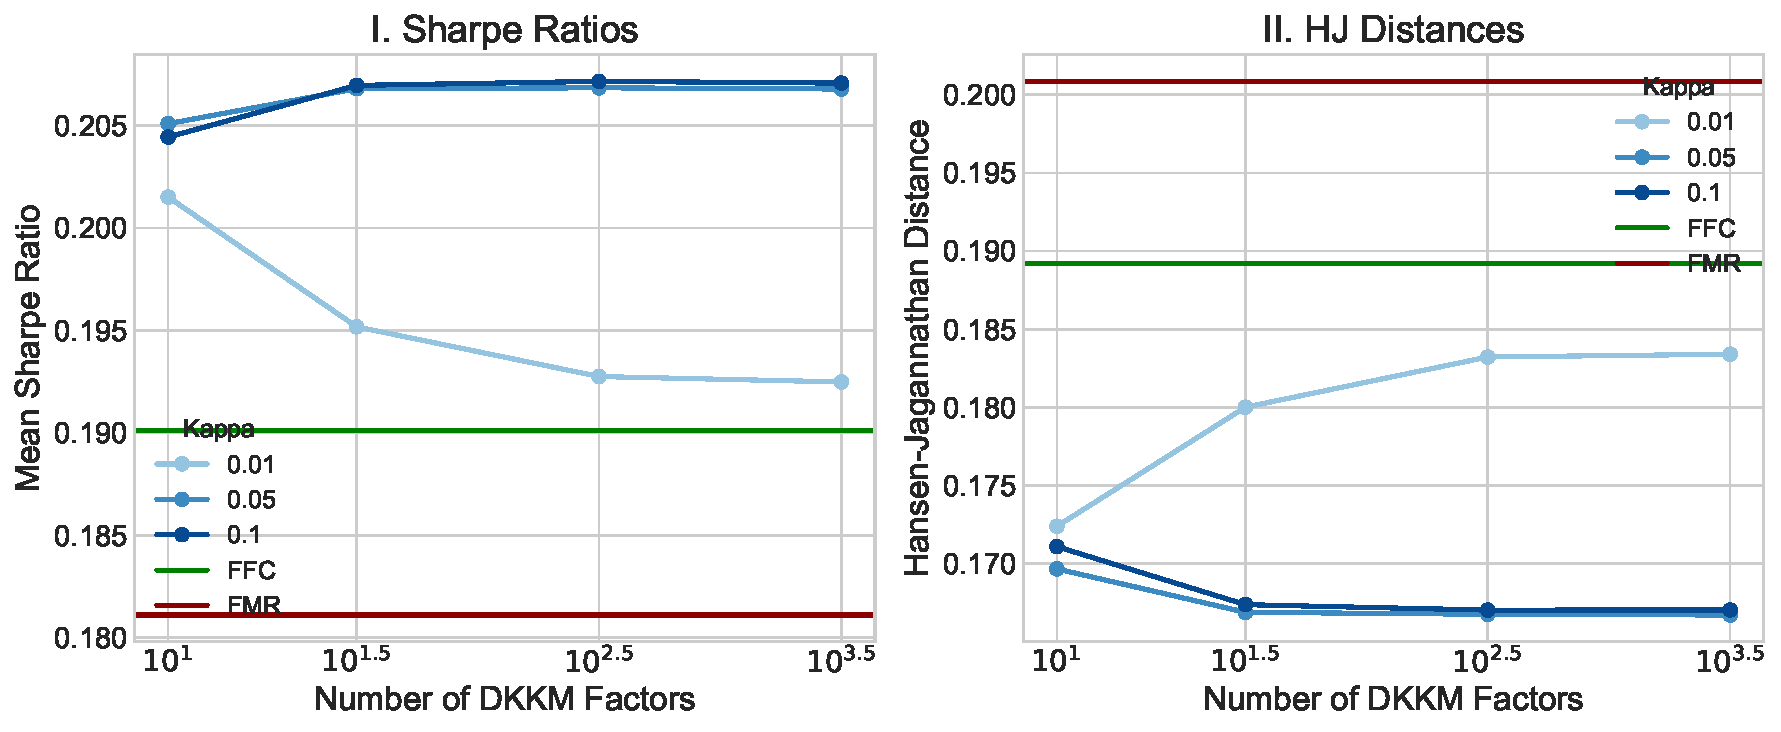
\includegraphics[width=\textwidth]{figures/dkkm_kp14.pdf}
\end{frame}

\begin{frame}{Gomes-Schmid Model}
  \centering
  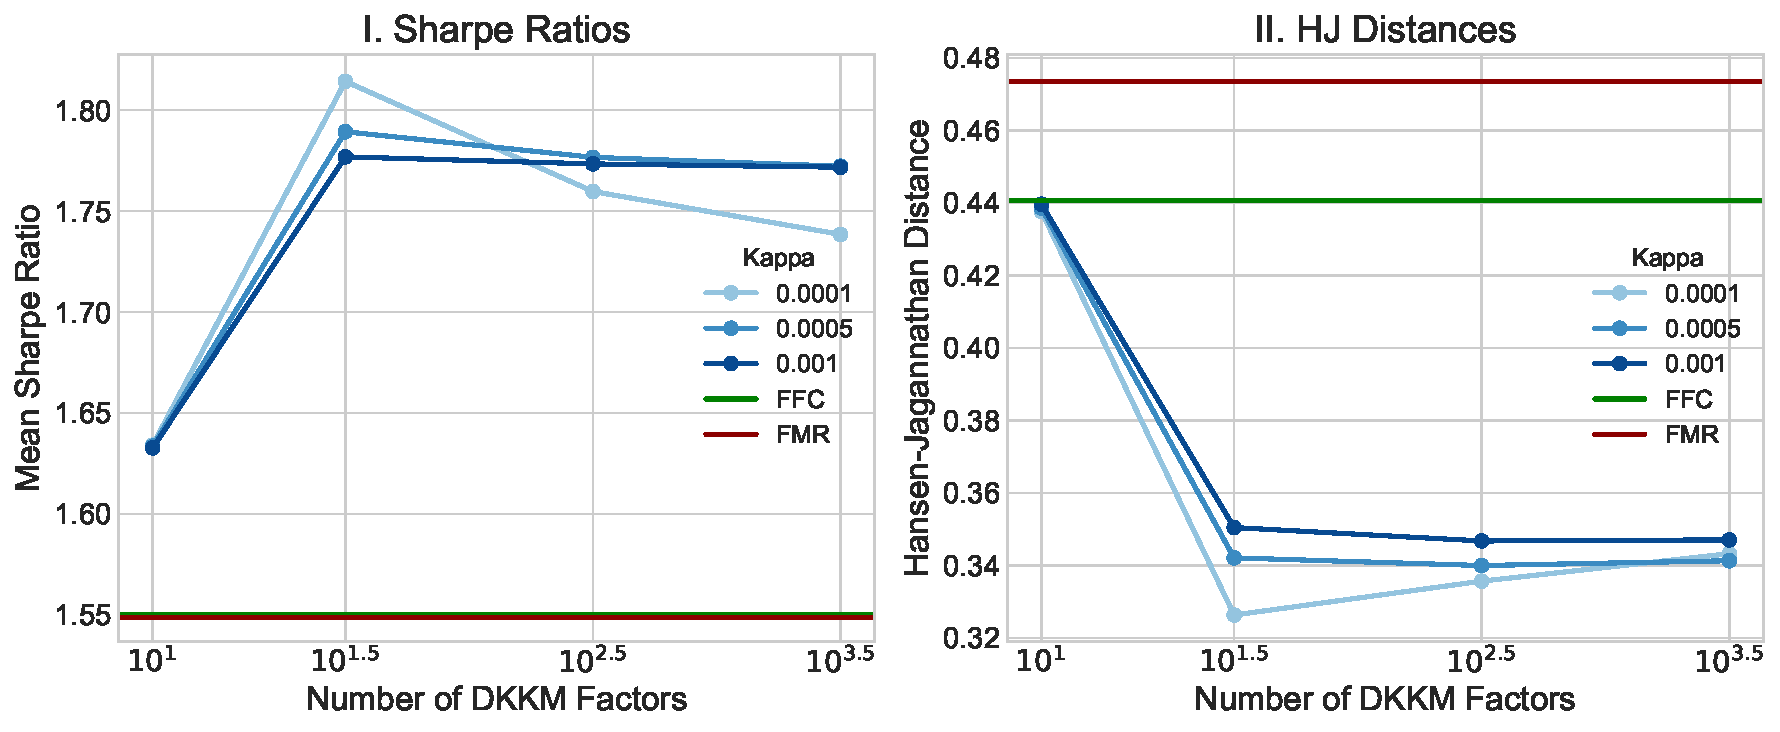
\includegraphics[width=\textwidth]{figures/dkkm_gs21.pdf}
\end{frame}

\begin{frame}{Sharpe Ratios in Excess of FFC: BGN Model}
  \centering
  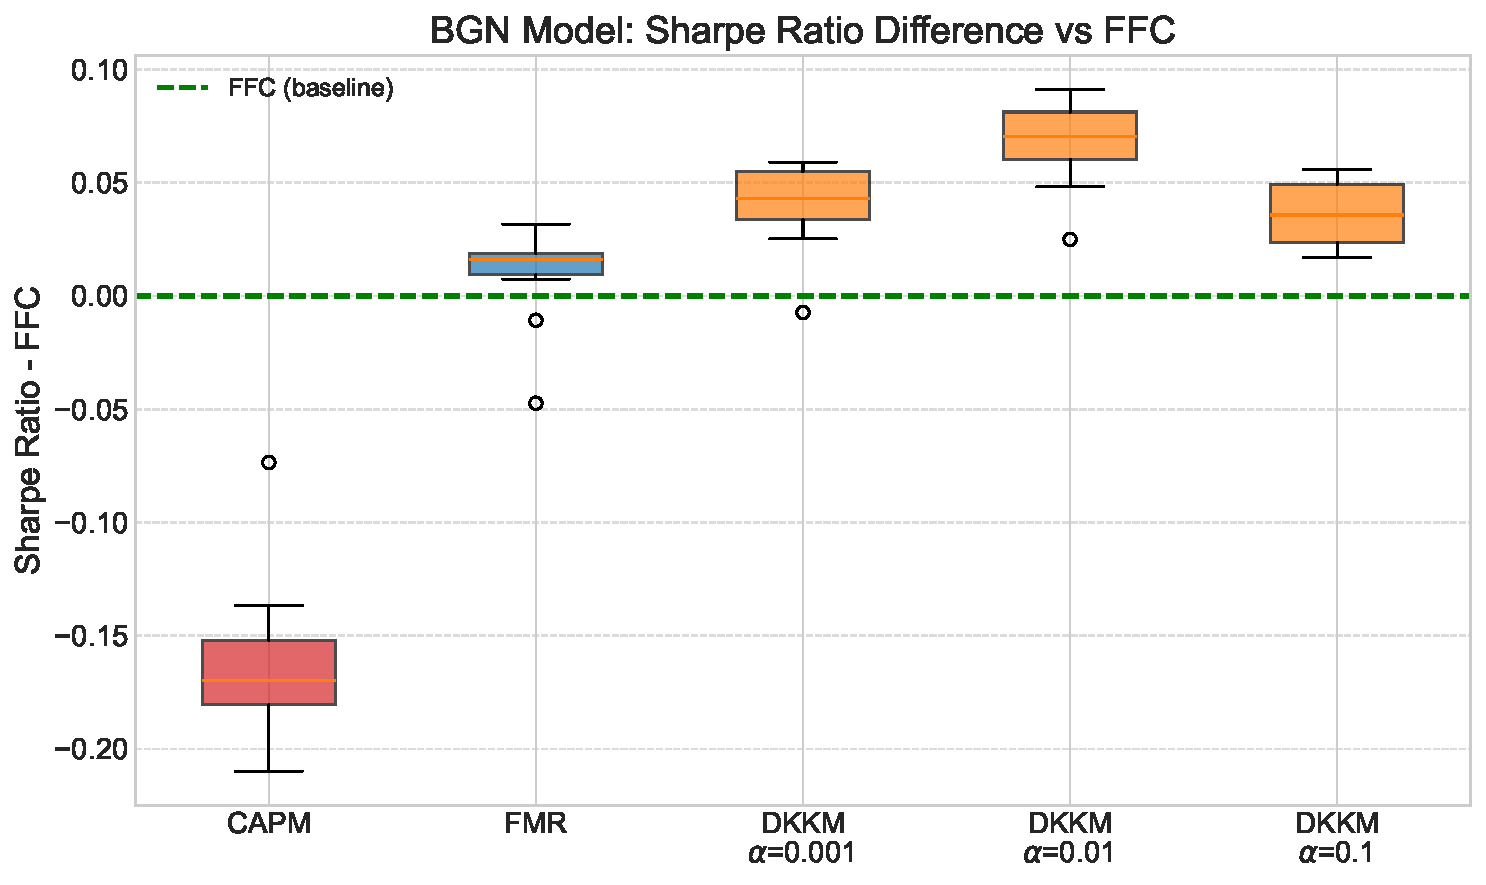
\includegraphics[height=0.85\textheight]{figures/sharpe_boxplot_bgn.pdf}
\end{frame}

\begin{frame}{Sharpe Ratios in Excess of FFC: KP Model}
  \centering
  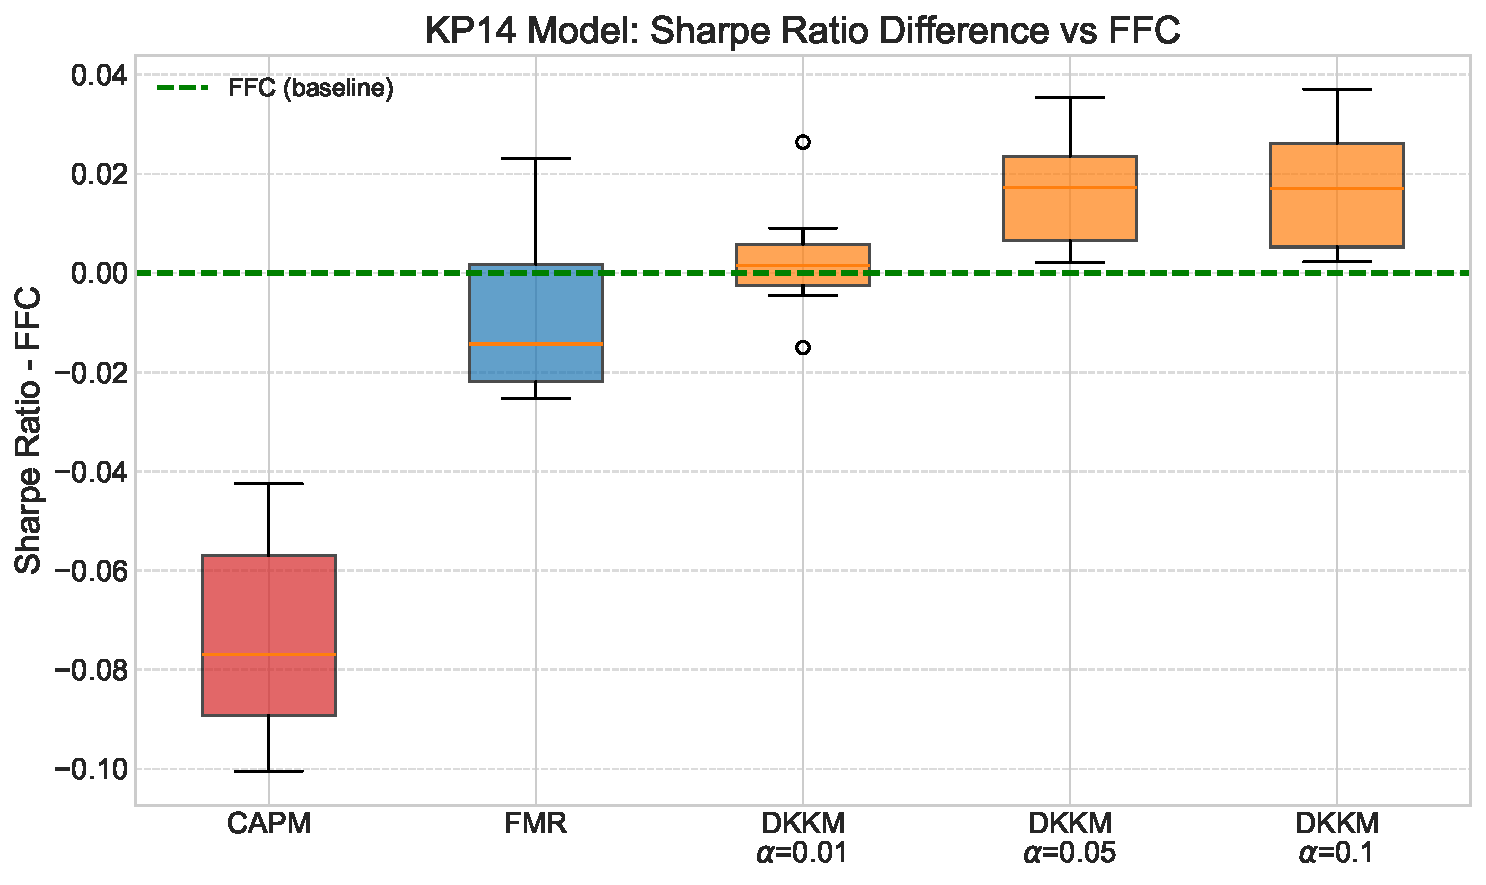
\includegraphics[height=0.85\textheight]{figures/sharpe_boxplot_kp14.pdf}
\end{frame}

\begin{frame}{Sharpe Ratios in Excess of FFC: GS Model}
  \centering
  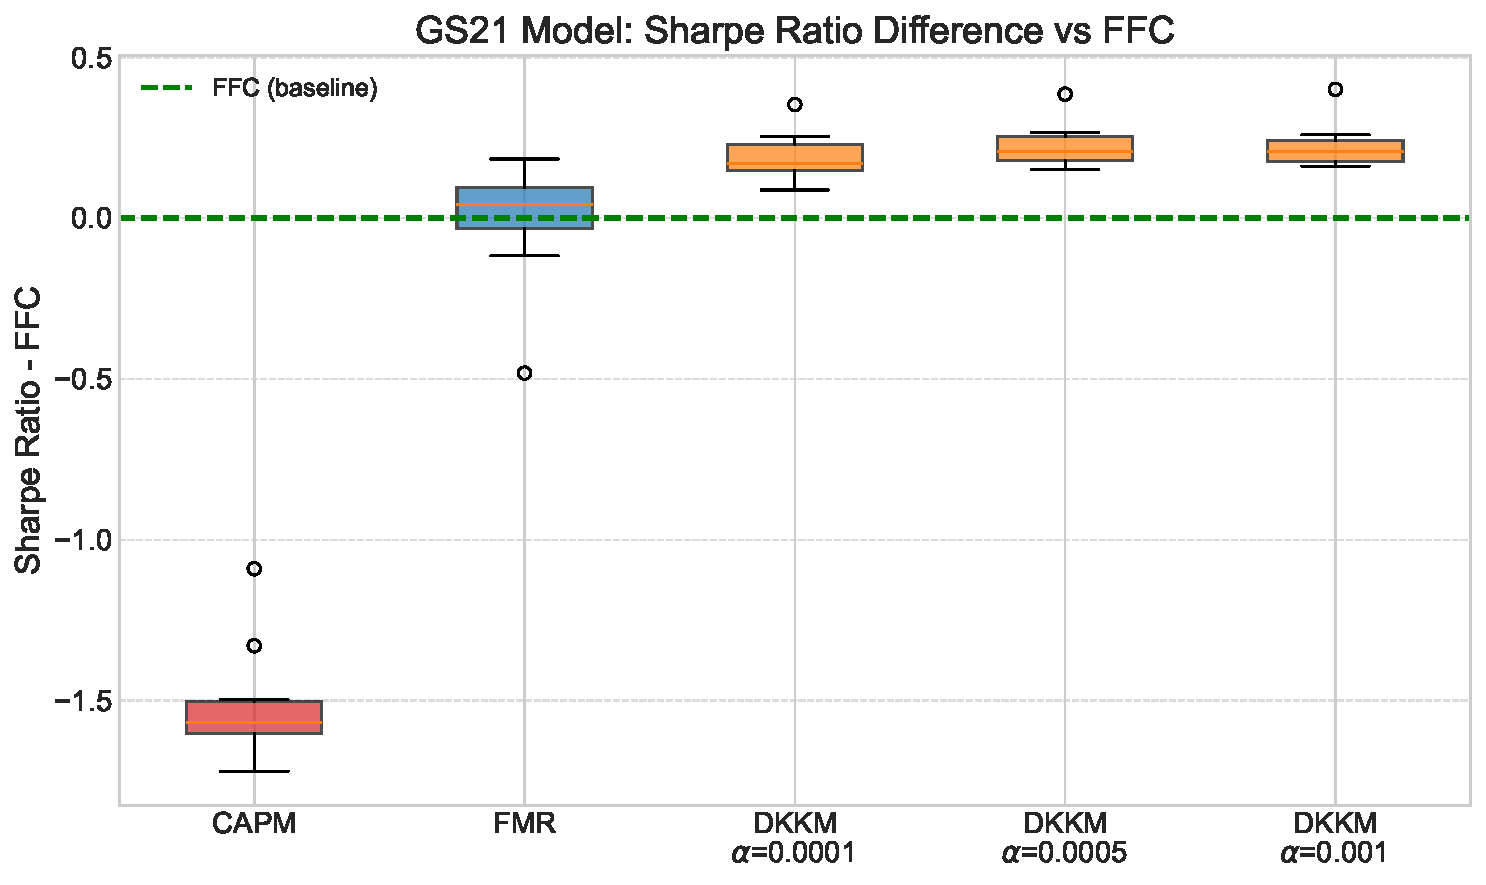
\includegraphics[height=0.85\textheight]{figures/sharpe_boxplot_gs21.pdf}
\end{frame}

\begin{frame}{HJ Distance in Excess of FFC: BGN Model}
  \centering
  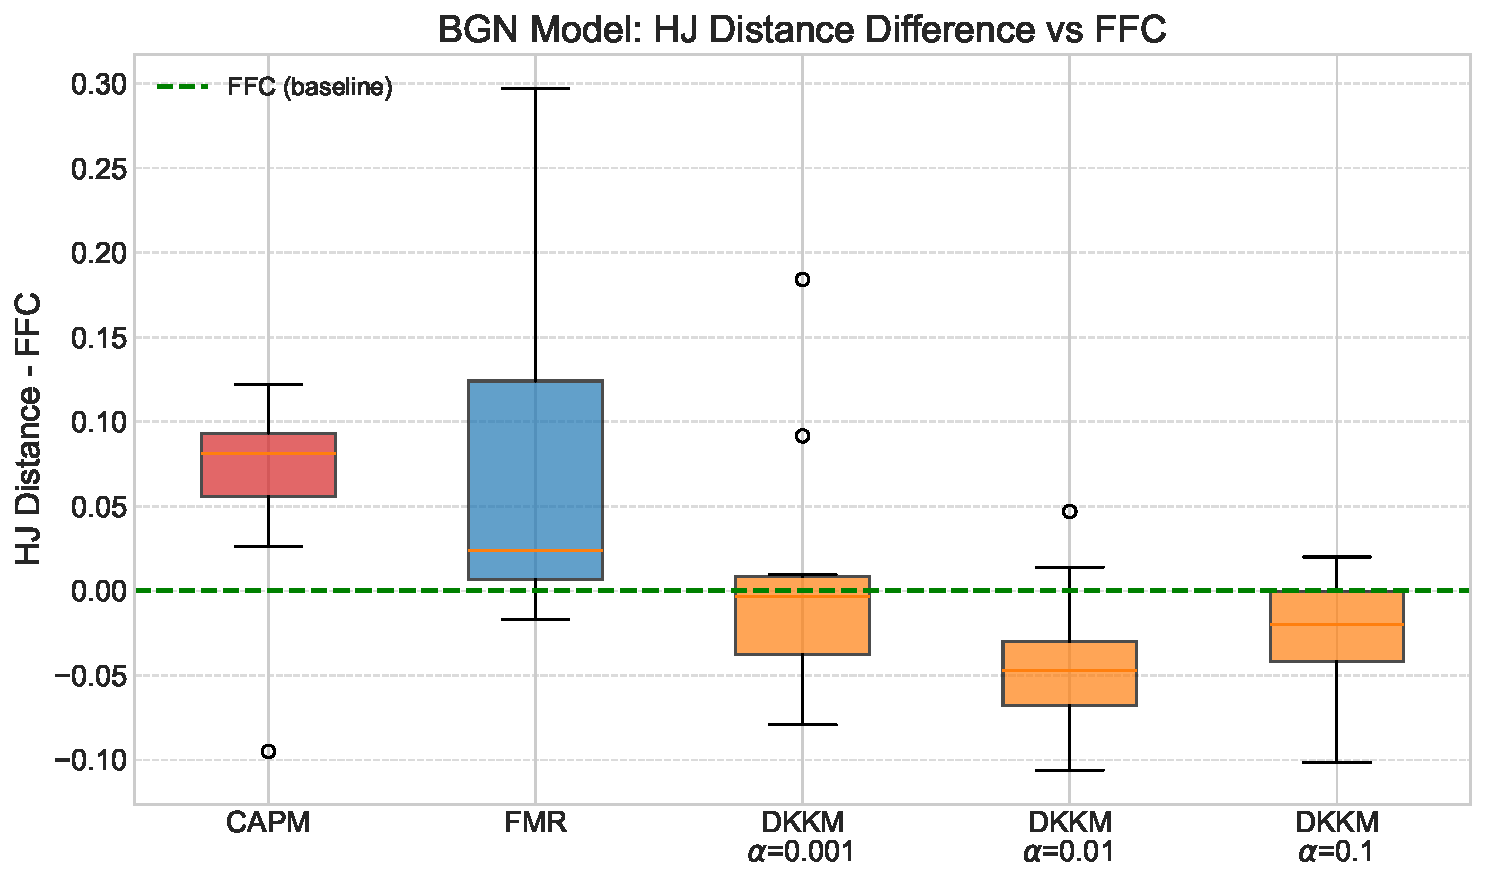
\includegraphics[height=0.85\textheight]{figures/hjd_boxplot_bgn.pdf}
\end{frame}

\begin{frame}{HJ Distance in Excess of FFC: KP Model}
  \centering
  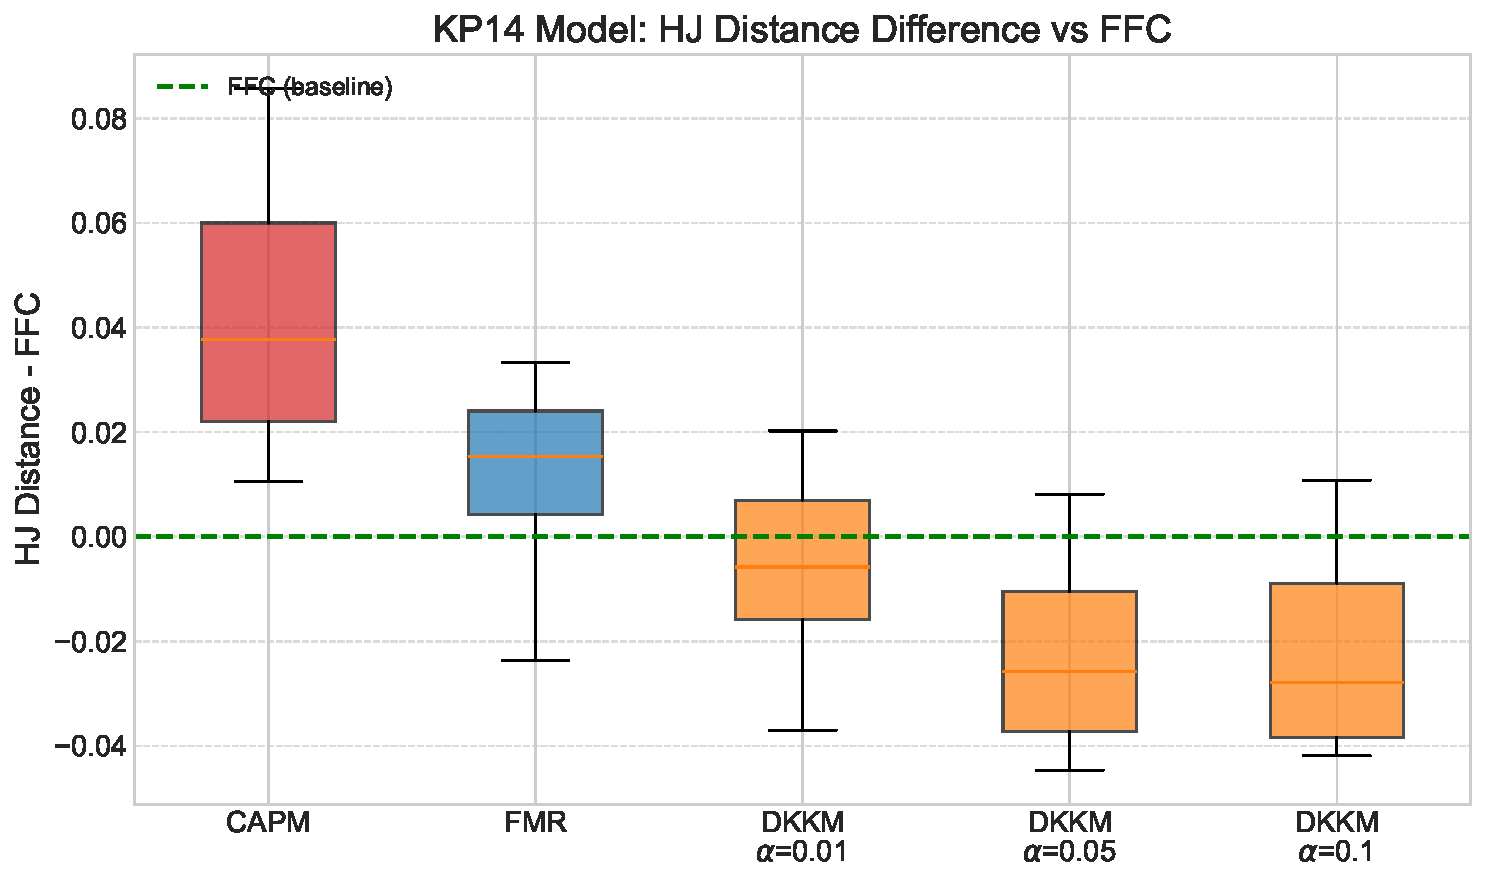
\includegraphics[height=0.85\textheight]{figures/hjd_boxplot_kp14.pdf}
\end{frame}

\begin{frame}{HJ Distance in Excess of FFC: GS21}
  \centering
  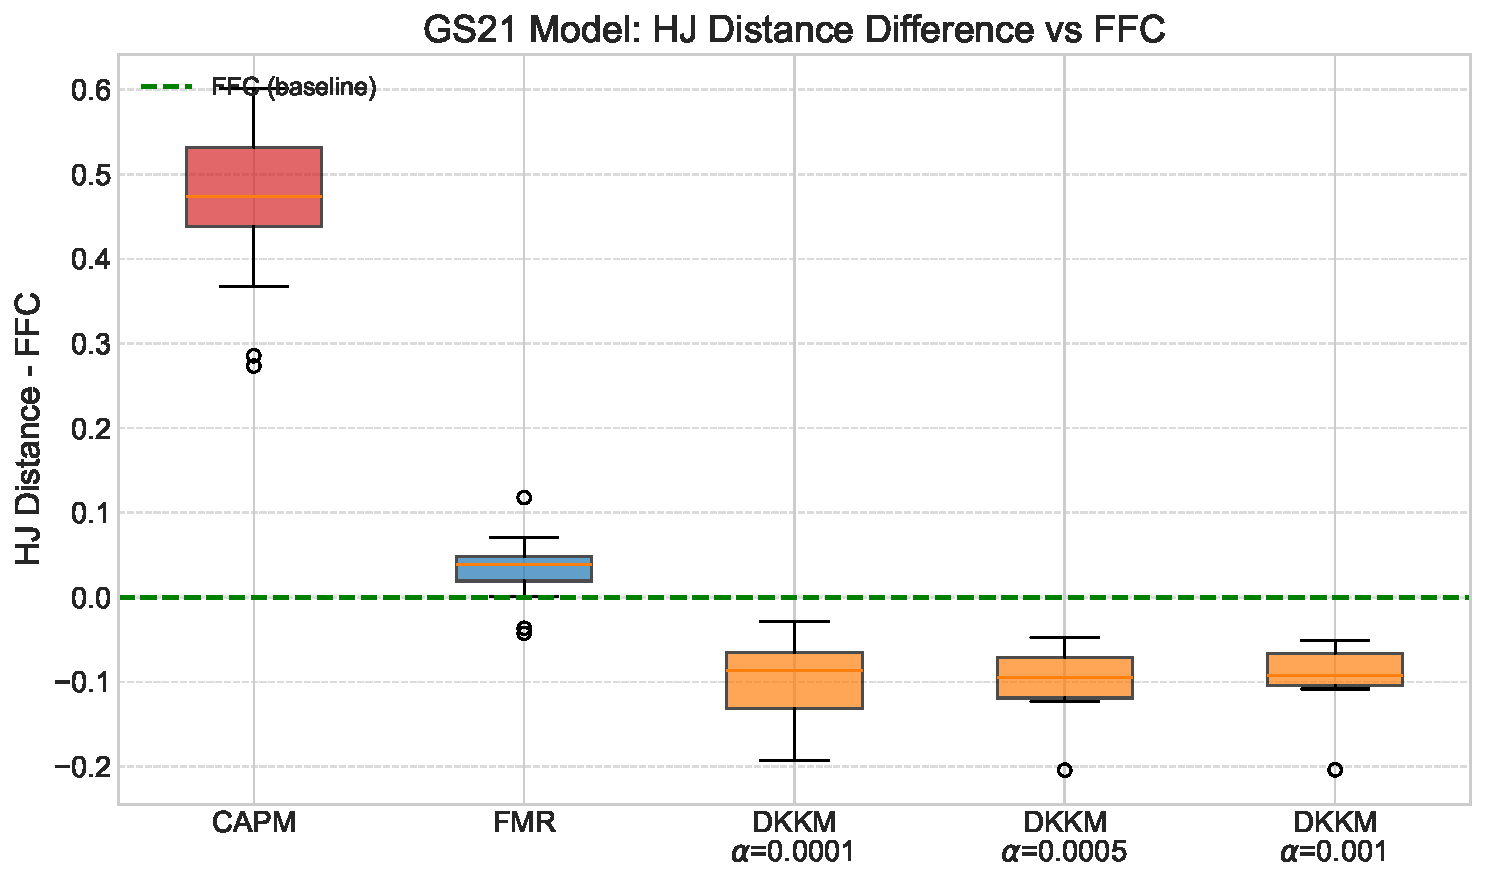
\includegraphics[height=0.85\textheight]{figures/hjd_boxplot_gs21.pdf}
\end{frame}

\begin{frame}{Statistical Tests: Sharpe Ratios}
DKKM (best $\alpha$, 3600 factors) vs other methods

\vspace{0.3cm}
Paired $t$-tests across simulation panels (one-tailed)
  \centering

  \vspace{0.3cm}
  \begin{tabular}{l c c c c c c c c c}
\toprule
& \multicolumn{3}{c}{vs CAPM} & \multicolumn{3}{c}{vs FFC} & \multicolumn{3}{c}{vs FMR} \\
\cmidrule(lr){2-4} \cmidrule(lr){5-7} \cmidrule(lr){8-10}
Model & Diff & $t$ & $p$ & Diff & $t$ & $p$ & Diff & $t$ & $p$ \\
\midrule
BGN & 0.232 & 19.5 & $<$0.001 & 0.067 & 12.6 & $<$0.001 & 0.058 & 9.5 & $<$0.001 \\
KP14 & 0.091 & 29.9 & $<$0.001 & 0.017 & 5.0 & $<$0.001 & 0.026 & 4.6 & $<$0.001 \\
GS21 & 1.751 & 45.4 & $<$0.001 & 0.222 & 11.8 & $<$0.001 & 0.223 & 3.4 & 0.003 \\
\bottomrule
\end{tabular}

  \vspace{0.3cm}
  \raggedright
  \small Positive diff = DKKM has higher Sharpe ratio
\end{frame}

\begin{frame}{Statistical Tests: HJ Distance}
DKKM (best $\alpha$, 3600 factors) vs other methods

\vspace{0.3cm}
Paired $t$-tests across simulation panels (one-tailed)
  \centering

  \vspace{0.3cm}
  \begin{tabular}{l c c c c c c c c c}
\toprule
& \multicolumn{3}{c}{vs CAPM} & \multicolumn{3}{c}{vs FFC} & \multicolumn{3}{c}{vs FMR} \\
\cmidrule(lr){2-4} \cmidrule(lr){5-7} \cmidrule(lr){8-10}
Model & Diff & $t$ & $p$ & Diff & $t$ & $p$ & Diff & $t$ & $p$ \\
\midrule
BGN & -0.107 & 4.6 & $<$0.001 & -0.043 & 3.4 & 0.003 & -0.125 & 4.2 & $<$0.001 \\
KP14 & -0.064 & 23.7 & $<$0.001 & -0.023 & 4.7 & $<$0.001 & -0.034 & 6.3 & $<$0.001 \\
GS21 & -0.565 & 25.2 & $<$0.001 & -0.099 & 8.3 & $<$0.001 & -0.132 & 6.5 & $<$0.001 \\
\bottomrule
\end{tabular}

  \vspace{0.3cm}
  \raggedright
  \small Negative diff = DKKM has lower HJ distance (better)
\end{frame}


\begin{frame}[c]
  \centering
  \Huge Pricing 25 Size-BM Portfolios
\end{frame}

\begin{frame}{GRS Test for Pricing Errors}
\begin{itemize}
\item Regress each of 25 size-BM portfolio returns on factor model return:
$$R_i = \alpha_i + \beta_i F + \varepsilon_i$$
\item GRS statistic tests $H_0: \alpha_1 = \cdots = \alpha_{25} = 0$
$$\text{GRS} = \frac{T-N-1}{N} \cdot \frac{1}{1+\text{SR}_F^2} \cdot \alpha'\Sigma^{-1}\alpha$$
\item Key metric: 
$$\alpha'\Sigma^{-1}\alpha = \text{max Sharpe ratio of} R-F\beta = \alpha + \varepsilon$$
\item Under $H_0$: GRS $\sim F(N, T-N-1)$
\end{itemize}
\end{frame}

\begin{comment}
\begin{frame}{Pricing Errors: BGN Model}
  \centering
  \begin{tabular}{lrrr}
\toprule
 & $\alpha'\Sigma^{-1}\alpha$ & GRS & $p$-value \\
\midrule
FFC & 0.168 & 1.962 & 0.046 \\
FMR & 0.192 & 2.260 & 0.009 \\
CAPM & 0.260 & 3.327 & 0.000 \\
DKKM ($\alpha=0.001$) & 0.144 & 1.604 & 0.150 \\
DKKM ($\alpha=0.01$) & 0.133 & 1.466 & 0.199 \\
DKKM ($\alpha=0.1$) & 0.160 & 1.821 & 0.036 \\
\bottomrule
\end{tabular}


  \vspace{0.3cm}
  \raggedright
  \small Lower $\alpha'\Sigma^{-1}\alpha$ and GRS = better pricing of 25 portfolios
\end{frame}

\begin{frame}{Pricing Errors: KP14 Model}
  \centering
  \begin{tabular}{lrrr}
\toprule
 & $\alpha'\Sigma^{-1}\alpha$ & GRS & $p$-value \\
\midrule
FFC & 0.085 & 1.030 & 0.465 \\
FMR & 0.083 & 1.009 & 0.477 \\
CAPM & 0.099 & 1.228 & 0.267 \\
DKKM ($\alpha=0.001$) & 0.090 & 1.111 & 0.361 \\
DKKM ($\alpha=0.01$) & 0.080 & 0.978 & 0.514 \\
DKKM ($\alpha=0.1$) & 0.079 & 0.956 & 0.544 \\
\bottomrule
\end{tabular}


  \vspace{0.3cm}
  \raggedright
  \small Lower $\alpha'\Sigma^{-1}\alpha$ and GRS = better pricing of 25 portfolios
\end{frame}

\begin{frame}{Pricing Errors: GS21 Model}
  \centering
  \begin{tabular}{lrrr}
\toprule
 & $\alpha'\Sigma^{-1}\alpha$ & GRS & $p$-value \\
\midrule
FFC & 0.766 & 3.809 & 0.077 \\
FMR & 0.960 & 5.419 & 0.007 \\
CAPM & 2.500 & 33.229 & 0.000 \\
DKKM ($\alpha=0.001$) & 0.597 & 2.260 & 0.223 \\
DKKM ($\alpha=0.01$) & 0.623 & 2.567 & 0.180 \\
\bottomrule
\end{tabular}


  \vspace{0.3cm}
  \raggedright
  \small Lower $\alpha'\Sigma^{-1}\alpha$ and GRS = better pricing of 25 portfolios
\end{frame}

\end{comment}
\begin{frame}{$\alpha'\Sigma^{-1}\alpha$ in Excess of FFC: BGN Model}
  \centering
  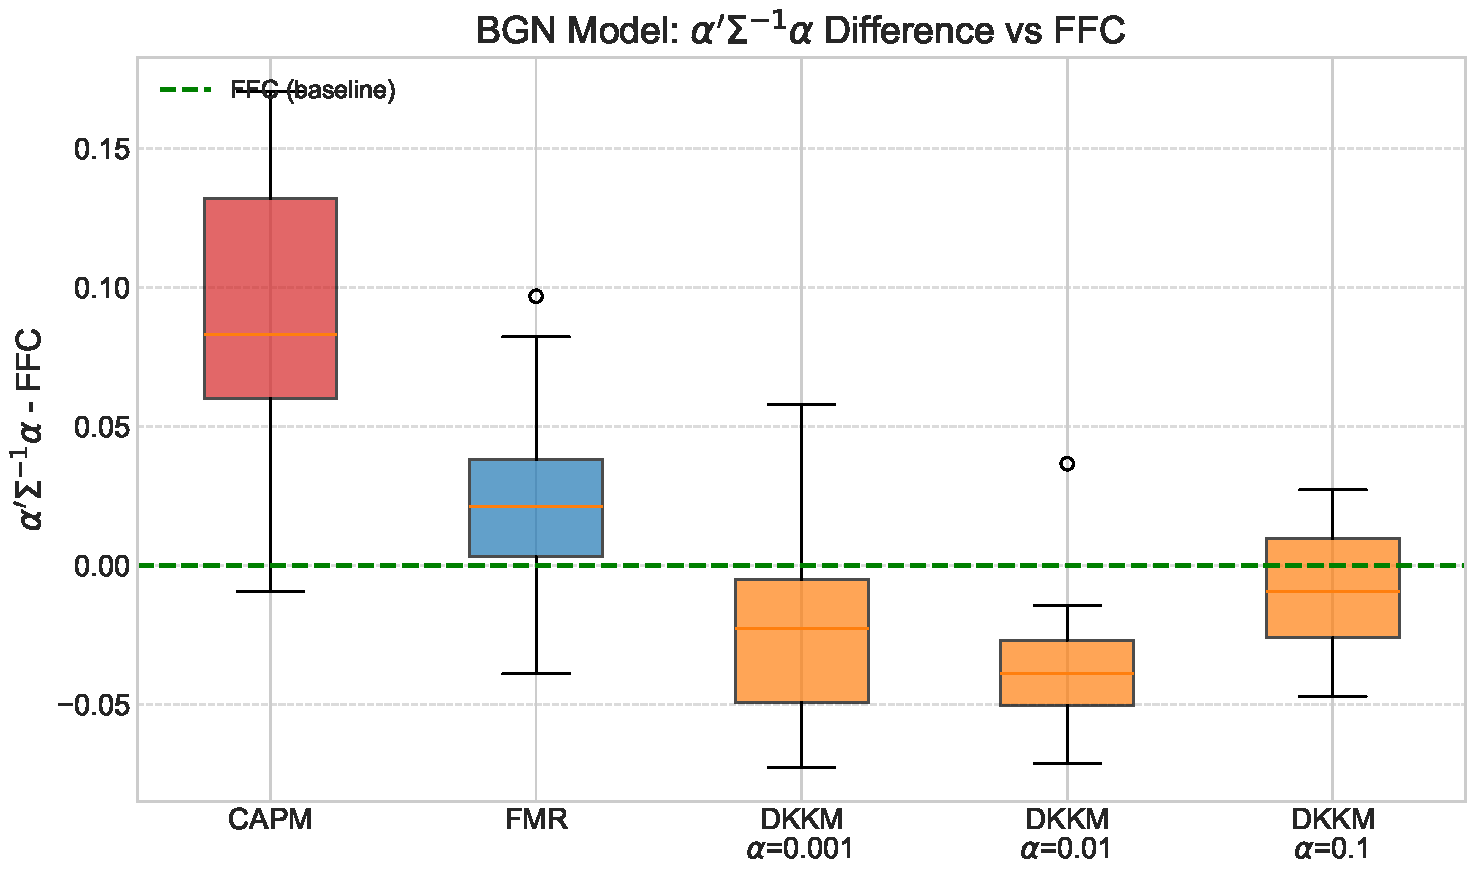
\includegraphics[height=0.85\textheight]{figures/alpha_quad_boxplot_bgn.pdf}
\end{frame}

\begin{frame}{$\alpha'\Sigma^{-1}\alpha$ in Excess of FFC: KP Model}
  \centering
  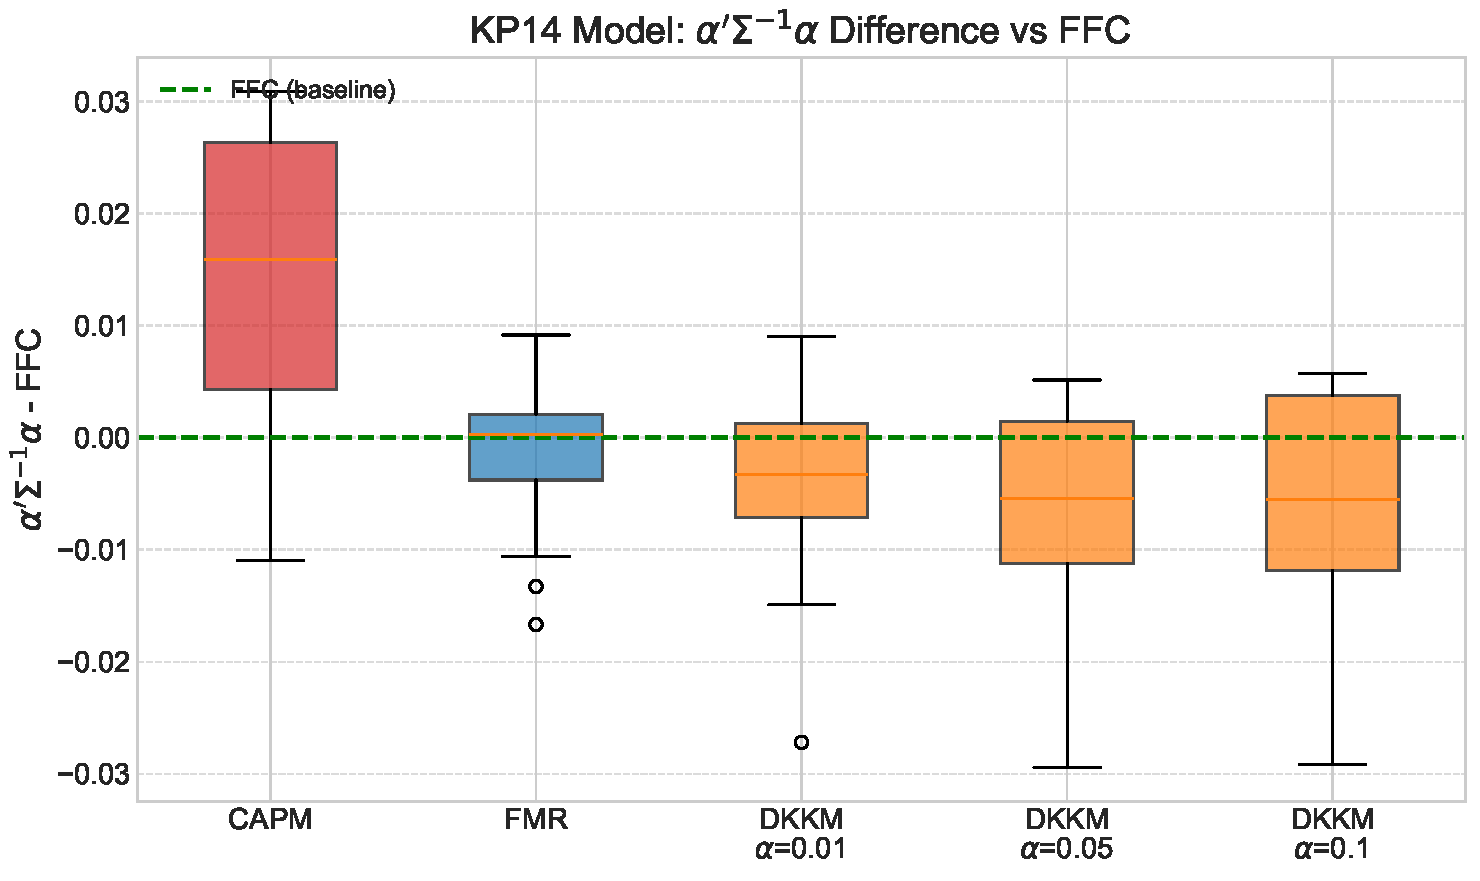
\includegraphics[height=0.85\textheight]{figures/alpha_quad_boxplot_kp14.pdf}
\end{frame}

\begin{frame}{$\alpha'\Sigma^{-1}\alpha$ in Excess of FFC: GS Model}
  \centering
  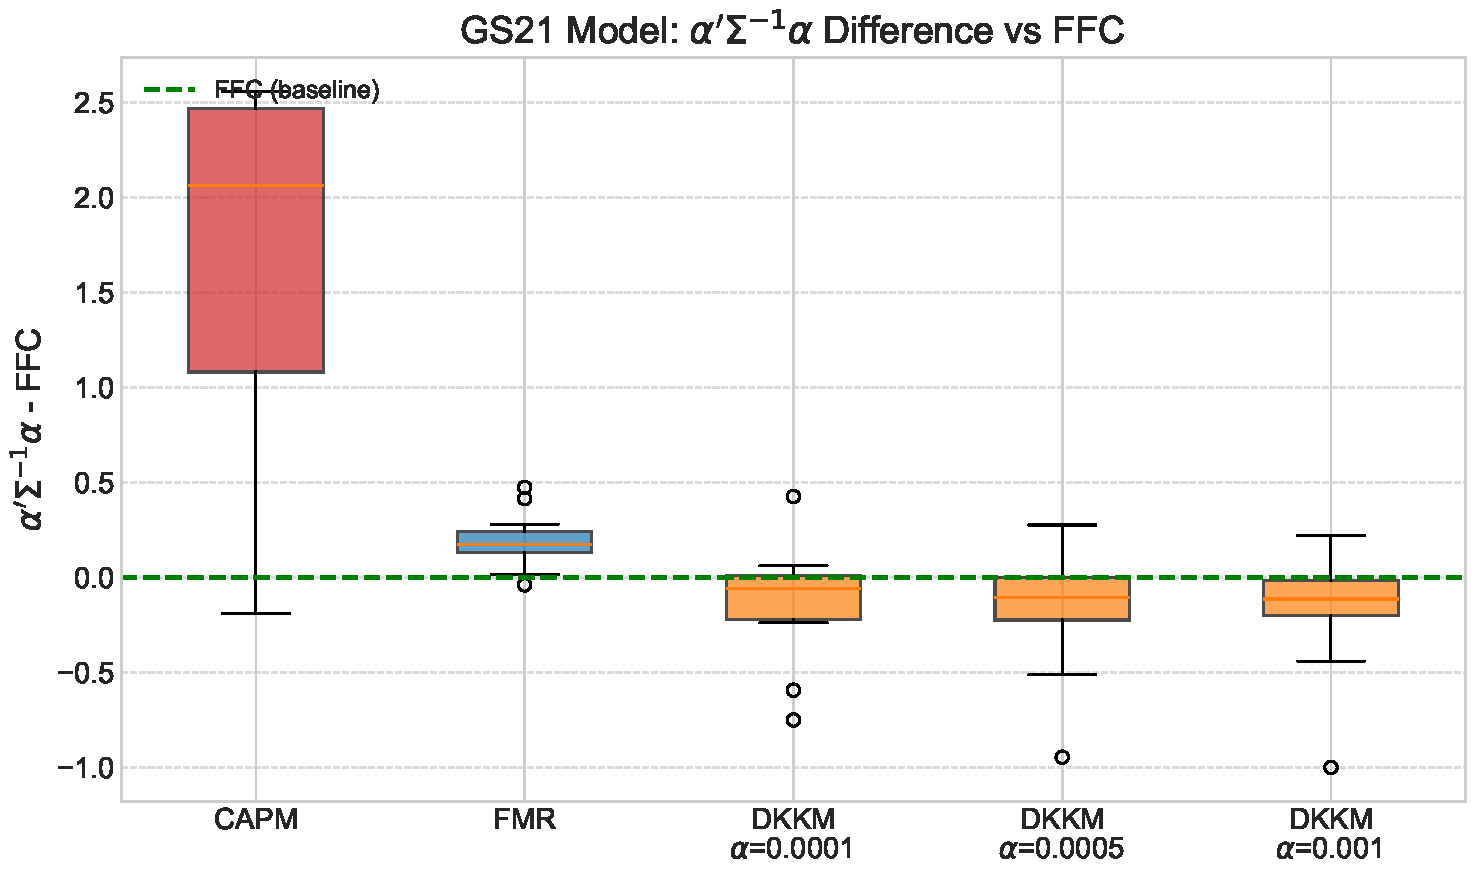
\includegraphics[height=0.85\textheight]{figures/alpha_quad_boxplot_gs21.pdf}
\end{frame}

\begin{frame}{Statistical Tests: $\alpha'\Sigma^{-1}\alpha$}
DKKM ($\alpha=0.001$, 3600 factors) vs other methods

\vspace{0.3cm}
Paired $t$-tests across simulation panels
  \centering

  \vspace{0.3cm}
  \begin{tabular}{lccc}
\toprule
 & FFC & FMR & CAPM \\
\midrule
BGN & -0.02 (-2.30)** & -0.05 (-3.49)*** & -0.12 (-8.62)*** \\
KP14 & 0.01 (1.55) & 0.01 (2.39)** & -0.01 (-2.17)* \\
GS21 & -0.17 (-1.91)* & -0.36 (-3.02)** & -1.90 (-7.33)*** \\
\bottomrule
\end{tabular}


  \vspace{0.3cm}
  \raggedright
  \small Format: diff ($t$-stat). Negative diff = DKKM has lower pricing errors (better). \\
  \small *$p<0.10$, **$p<0.05$, ***$p<0.01$
\end{frame}

\begin{frame}{Statistical Tests: GRS Statistic}
DKKM ($\alpha=0.001$, 3600 factors) vs other methods

\vspace{0.3cm}
Paired $t$-tests across simulation panels
  \centering

  \vspace{0.3cm}
  \begin{tabular}{lccc}
\toprule
 & FFC & FMR & CAPM \\
\midrule
BGN & -0.36 (-2.65)** & -0.66 (-3.71)*** & -1.72 (-11.01)*** \\
KP14 & 0.08 (1.64) & 0.10 (2.36)** & -0.12 (-2.18)* \\
GS21 & -1.55 (-2.61)** & -3.16 (-2.85)** & -30.97 (-12.96)*** \\
\bottomrule
\end{tabular}


  \vspace{0.3cm}
  \raggedright
  \small Format: diff ($t$-stat). Negative diff = DKKM has lower GRS (better). \\
  \small *$p<0.10$, **$p<0.05$, ***$p<0.01$
\end{frame}

\begin{frame}{Conclusion}
\begin{itemize}
\item In theoretical economies, we know the true SDF, so can calculate the true errors of pricing models.
\item Provides a laboratory for evaluating models
\item Results:
\begin{enumerate}
\item More complexity is better
\item Complexity beats standard models
\end{enumerate}
\item This is true even in simple economies!
\end{itemize}
\end{frame}

\end{document}
